
\documentclass{report}
\usepackage{geometry}
%\usepackage{layout}
\usepackage{graphicx}

\setlength{\headsep}{1pt}


\begin{document}

\title{Collection and Recording of Data For the Study and Improvement of Sky Diving and Formation forming}
\author{Michael Mason}

\maketitle


\begin{abstract}
When skydiving the ability to record data of the jump is essential when jumping in formation. With the use of inertial measurement units (IMU) it is possible to gain a better understanding of the technique used and improve on form. With the use of sensing equipment such as ; Magnetometer, accelerometer, gyroscope it is possible to get accurate results of pitch, yaw and roll. The choice of a good micro-controller will determine the over all efficiency.
Storing this data and being able to access it either between jumps or after a day of jumping is essential. Making this easy for the user to attain will be looked at in the form of SD cards and direct link. Blue-tooth will also be discussed.
Making the device energy efficient and possibilities of scavenging energy from wind and sun will be discussed. During the project, the price of materials will be in the forefront of thought, ensuring that a good price to efficiency ratio will be met.

\end{abstract}

\tableofcontents



\chapter{Hardware Selection and Design}
Choosing the correct hardware will define the overall practicality of the project. Several factors have to be taken into consideration when selecting hardware such as functionality, connections, power consumption and size with many more. These will be discussed in detail and compared to other products with indication why they were chosen over them. What storage is used for the device and the format in which it is stored in will be discussed
Both prototyping and final design will be discussed in separate stages to provide a structured design to the final product.
The three main sensing components that will be used will be a gyroscope, accelerometer and a magnetometer. Using all three allows for greater results. When combined together the accelerometer and gyroscope will work with each other to provide the pitch and roll. To receive the yaw result the manometer will be used.

\section{Breakout Board Prototype}
For the prototyping breakout board will be used. By creating the prototype using breakout boards it is possible to have a more practical and faster way to make the product. It will also be good to study the way that they are put together to then efficiently create the final product. A great advantage of using break out for the prototyping is that they include any resistors or capacitors that may be needed to reduce noise on the device. This will be considered when creating the final design, hopefully based on some ideas that the break out boards provide.
 
\subsection{Micro-controller}
The micro-controller is chosen due to the sensors that are needed. Available EEPROM memory is taken in to account to store system files. The micro controller that will be used for the prototype is PIC16F818. 
\begin{itemize}
\item 128 bytes of EEPROM data memory
\item 2 to 5.5 voltage
\item $i^2c$
\end{itemize}

\subsection{Gyroscope}
The gyroscope that will be used in the prototype will be the Triple-Axis Digital-Output Gyro ITG-3200 breakout board. By using the inter-integrated 
This particular model has been chosen due to the completeness of the device and it flexible power consumption rate.
\begin{itemize}
\item voltage range of 2.1V to 3.6V
\item Fast Mode $i^2c$ (400kHz) serial interface
\end{itemize}
\subsection{Accelerometer}
The triple axis MMA8452Q break out board will be sourced for the prototype. One of the great features of this particular device is the ability to stay in low power mode until told otherwise. This will save power and can be incorporated with possibly another embedded device such as the barometer or a simple switch to swap between power modes.
\begin{itemize}
\item ±2g/±4g/±8g dynamically selectable full-scale
\item I2C digital output interface
\item 1.6 V to 3.6 V interface voltage
\end{itemize}

\subsection{Magnetometer}
Triple Axis Magnetometer Breakout - MAG3110 will be sourced for the magnetometer. This particular board comes with its own voltage regulator opposed to its main competitor, HMC5883L, which does not. This allows for a wider spectrum of voltage control .
\begin{itemize}
\item 1.95V to 3.6V Supply Voltage
\item 7-bit I2C address = 0x0E
\end{itemize}

\subsection{Barometer}
Barometric Pressure Sensor - BMP180 Breakout will be used to measure pressure. This will be used to measure the altitude of the device. 
\begin{itemize}
\item Digital two wire (I²C, TWI, "Wire")
\item Ultra-low power consumption - Flexible supply voltage range (1.8V to 3.6V)
\end{itemize}

\subsection{SD Card Reader}
SD cards are non volatile storage. This allows information to be stored even when the device is not under direct power. The ability to remove the storage device will allow the user to retrieve the data collected and upgrade the devices storage. The component used for prototyping will be Breakout Board for microSD Transflash. This product will also be sourced out for the final design.
To 

\subsection{Power}
The aim goal for the power is small and rechargeable. With this in mind the ANSMANN 3.7V Wire lead terminal has been chosen.
\begin{itemize}
\item 3.7v nominal
\item 2250mAh
\item Lithium-Ion
\end{itemize}



\section{Final Product Specification}

\subsection{Micro-controller}
The micro controller that will be used for the prototype is PIC16F818. This is the same micro controller that was used in the prototype. For its capabilities and its price it seem the most efficient. With having 128Bytes EEPROM memory it is possible to store the code for the device on here. It will then export the information that is collected straight of the micro sd card ready for the user to transport to a computer for retrieval. The micro-controller also has bi-directional I/O ports which allow for multiple $i^2c$ connections. It allows for selectable selectable frequencies, including 31.25 kHz, 125 kHz,250 kHz, 500 kHz, 1 MHz, 2 MHz, 4 MHz and 8 MHz from the RC oscillator. This will enable the ability to select the most efficient frequency and will save power usage. 
\begin{itemize}
\item 128 bytes of EEPROM data memory
\item 2 to 5.5 voltage
\item $i^2c$
\end{itemize}
\begin{center}
  \begin{tabular}{ | l | c | r |}
    \hline
    Amount & Price W/O VAT £ & Price £ \\ \hline
    1 & 1.58 & 1.90 \\ \hline
    10 & 1.33 & 1.60 \\ \hline
    100 & 1.22 & 1.46   \\ \hline
  \end{tabular}
\end{center}

\subsection{Gyroscope and Accelerometer}
STMICROELECTRONICS - LSM330DLC functionas as both gyroscope and accelerometer. As opposed to the prototype model this unit contains both. The advantage of this is the connections used will be less. It is also by far and large the cheapest that has been sought out and works well with the voltages needed and the micro controller. It does not have any extra features such as stand by mode or a sleep mode. Is supported by a $i^2c$ connector. This particular model has the ability to change from low power mode to optimal mode when it is in free fall. This is not going to be exploited in this model but may be considered for the MKII
\begin{itemize}
\item 2.4 - 3.6 voltage 
\item Gyroscope -  ± 250°/s, ± 500°/s, ± 2000°/s
\item Accelerometer - ± 2g, ± 4g, ± 8g, ± 16g
\item SMT surface mount 
\item Triple axis both
\end{itemize}

\begin{center}
  \begin{tabular}{ | l | c | r |}
    \hline
    Amount & Price W/O VAT £ & Price £ \\ \hline
    1 & 4.69 & 5.63 \\ \hline
    10 & 3.81 & 4.75 \\ \hline
    100 & 3.28& 3.94  \\ \hline
  \end{tabular}
\end{center}

\subsection{Magnetometer}
MEMSIC - MMC33160MT magnetometer has been selected. This particular device takes readings from the X, Y, and the Z axis as measured data. Being connected to the micro-processor directly from the $i^2c$ bus, it eliminates the need for any A/D converters. 

\begin{itemize}
\item $accuracy^2$ ~ min = +-2.0 / max +- 5.0 degrees 
\item voltage 1.6 - 3.7 volts. Typical 1.6
\item -8/+8 gauss
\item SMT surface mount 
\end{itemize}

\begin{center}
  \begin{tabular}{ | l | c | r |}
    \hline
    Amount & Price W/O VAT £ & Price with VAT £ \\ \hline
    1 & 6.90 & 8.28 \\ \hline
    10 & 5.30 & 6.36 \\ \hline
    100 & 4.32 & 5.18 \\ \hline
	\end{tabular}
\end{center}

\subsection{Barometer}
MEMS-LPS331AP has been chosen. Due to its ability to operate at -40 degrees this particular model is better than some other that were looked at that would not operate below 0 degrees. It has a operating voltage of around 1.7 volts which matched nicely with the other sensing components. With both SPI and $i^2c$ I/O, makes it extremely practical for the micro-controller used. Its ability to work to 35,000 feet means that it has plenty of operating space for this product, which has been designed with 10,000 feet in mind.

\begin{itemize}
\item 1.71 V to 3.6 V
\item Operating temperature -40 - +85 degrees 
\item 260 to 1260 mbar absolute pressure range
\end{itemize}

\begin{center}
  \begin{tabular}{ | l | c | r |}
    \hline
    Amount & Price W/O VAT £ & Price with VAT £ \\ \hline
    1 & - & 3.21 \\ \hline
    10 & - & 2.58 \\ \hline
    100 & - & 2.29 \\ \hline
	\end{tabular}
\end{center}

\subsection{SD Reader}
SD reader 798-DM3CSSF has been chosen as the storage of the device. Due to its large capacity and small, light weight size its a great source of storage. Micro SD typically operates at 100mb read and write speed and allows for flexibility in the amount of data that is written. 0-4 lines can be done simultaneously depending on the requirements and voltage regulations. Only one line will need to be written at a time and comma spacing will be used to separate the data for each separate recording while in the free fall. 
\begin{itemize}
\item Can retain data without power
\item Are rewritable
\item Will store large volumes of data on jumps
\end{itemize}

\begin{center}
  \begin{tabular}{ | l | c | r |}
    \hline
    Amount & Price W/O VAT £ & Price with VAT £ \\ \hline
    1 & - & 1.21 \\ \hline
    10 & - & 1.00 \\ \hline
    100 & - & 0.618 \\ \hline
	\end{tabular}
\end{center}

\subsubsection{MicroSd Card}
A 2GB Micro SD Flash memory card will be supplied with the unit. This will have an operating voltage between 2-3.7v and will use 100 $\mu A$.
One unit will cost £4.99 and will be supplied with the device.


\subsection{Battery}
 BAK 103450AR2 wire lead type has been chosen. As used in the prototype, Having researched further into the price and size this battery is most suitable. The advantages of lithium ion mean that this particular battery means that it will not need prolonged priming when bought One normal charge will suffice. This will help with sales of the device at the jump centres as they can be used when purchased.
\begin{itemize}
\item 3.7v nominal
\item 1.8Ah
\item Lithium-Ion
\end{itemize}

\begin{center}
  \begin{tabular}{ | l | c | r |}
    \hline
    Amount & Price W/O VAT £ & Price with VAT £ \\ \hline
    1 & - & 16.96 \\ \hline
    20 & - & 15.94 \\ \hline
	\end{tabular}
\end{center}

\subsubsection{Power Requirements} 
\begin{center}
\begin{tabular}{ | l | c | c | c | c | r |}
\hline
  Components&Current $\mu A$&Amp hours&Voltage&Energy\\ \hline
   Micro-Controller& 87 & 0.3132 & 2& 0.6624  \\ \hline
   Magnetometer& 900 & 3.24 & 3.6   &11.66  \\ \hline
   Accelerometer/Gyroscope&6111 & 2.1996 &1.8    &39.59 \\ \hline
   SD card& 100 &0.36  & 3.6   & 1.29   \\ \hline
   Barometer&30  &0.108  &  1.8 & 0.19 \\ \hline
   Total&7228 &26.0208  & 3.6  &53.38  \\ \hline
  	\end{tabular}
\end{center}

Power requirements of each sensor have been taken as the maximum needed and used to calculate the total energy that will be used by the device. A total of 53.38  J of energy will be used by the device per hour. 

\subsection{Notification}
To notify the user of the current state of the product a single LED will be used, TruOpto High Intensity LED White. The benefits using one LED will be shown in the state diagram. When the device is on the LED will show a solid color. When the device is recording data it will flash at periodic intervals. As the data is not transferred from the device, but rather through the medium of a removable SD card, there is no need to indicate to the user if the device is transferring. Solid color = on, flashing light = recording. 
This also allows the device not to have a LED constantly on. If the flash was to be every 5 seconds, on a days worth of jumping this would save battery life.

\begin{center}
  \begin{tabular}{ | l | c | r |}
    \hline
    Amount & Price W/O VAT £ & Price with VAT £ \\ \hline
    1 & 0.476 & 0.572 \\ \hline
    10 & 0.368 & 0.266 \\ \hline
    100 & 0.256 & 0.307 \\ \hline
	\end{tabular}
\end{center}


\section{Size and Price}
The size of the product  has been given to the specification of 50mm × 30mm × 15mm. The device will be built around the largest component, the battery. This has the longest length of 50mm so will fit to the specification required.
The device price per unit will work out at £42.18 per unit. This is based on buying the components at less that 10 per unit.
\section{Description and Diagram of the Interconnections}

\begin{figure}[ht!]
\centering
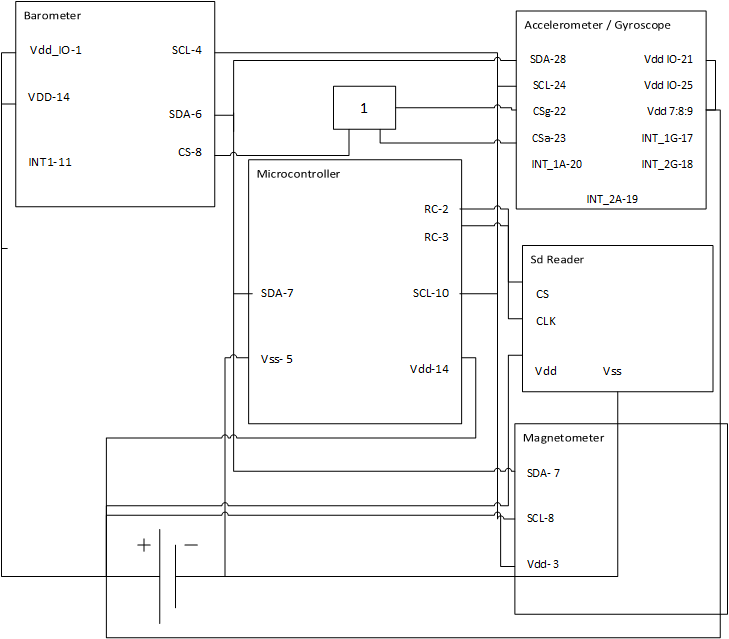
\includegraphics[width=115mm]{MainImage.png}
\caption{Diagram of the interconnections}
\label{overflow}
\end{figure}

\subsection{Reasons of Choice}
The reasons in choice for the type of serial bus was down to the flexibility and available parts. Building the project with $I2^C$ in mind allowed for a more straight forward approach in connecting to the micro-controller. Inter integrated circuit controller or $I2^C$ is more recent than SPI and has more flexibility in particular areas such as;

\begin{itemize}
\item Analogue to digital / digital to analogue conversion 
\item Use with memory chips such as EEPROM, RAM, FERAM, Flash
\item Use with other micro controller (may be required for MKII)
\end{itemize}

When information is requested from the device it is sent down the same bus. 7 bits are used in the address and the remaining bit is used to indicate weather the master wished to read or write the data. This will look somthing like [xxxxxxx1]

One of the main disadvantages that $I2^C$ has in comparison to SPI is the data transfer rate of up to 10MHz as opposed to the normal rate of 400KHz. 

As seen in diagram 1.1 the basic connections for all the main sensory equipment can be seen. Due to the use of the same $i^2c$ connection it is possible to connect to the same pin. 


\newpage
\chapter{Control Algorithm and Software}


\section{Operating modes}
The device will try to be as simplistic as possible to use. By having the main states; Off, Standby and Recording, it will use LED to indicate what the device is doing. As the device is in standby mode it will be in low power mode ready  to move to the recording state. When in the recording state, transfer of the data collected will be wrote straight to the microSD card. The LED will be a solid colour of yellow when the device is on. To indicate that the device is recording data the LED will be flash the same yellow. Along side the yellow light a flashing red will indicate that data is being wrote to the microSD card. This means that the user will see a red/yellow intermittent flash when in the jump. This system has be inspired by the iPod shuffle that does not have a screen but is able to indicate its current state very efficiently.

\section{Major Functions}
The micro-controller will have 4 sensory equipment. Each one will collect information and send it direct to the micro-controller where it will then be written to the microSD card. The four main data collecting functions will be;

\begin{itemize}
\item $COL$-$BARO$
\item $COL$-$GYRO$
\item $COL$-$MAG$
\item $COL$-$ACC$
\end{itemize}

\subsubsection{$COL$-$BARO$}
The barometer will collect data on the pressure of the surroundings of the device current hight. This will be measured in bar. Some mathematics will have to be done on the device to convert to pascals so that the user can then work out in feet the hight they were at. Untill the device is tested this will be hard to know if there is enough time to do the maths and right to the microSD card at the same time. 
\subsubsection{$COL$-$GYRO$}
The gyroscope will collect three axis information based on the orientation. This will be sent to the micro-controller and the wrote to the microSD. The data will be raw from the sensor and will be processed on the same line using comma spacing.
\subsubsection{$COL$-$MAG$}
The magnetometer will collect three axis information based on the orientation. This will be sent to the micro-controller and the wrote to the microSD. The data will be raw from the sensor and will be processed on the same line using comma spacing.
\subsubsection{$COL$-$ACC$}
The accelerometer will collect three axis information based on the orientation. This will be sent to the micro-controller and the wrote to the microSD. The data will be raw from the sensor and will be processed on the same line using comma spacing.



\begin{figure}[ht!]
\centering
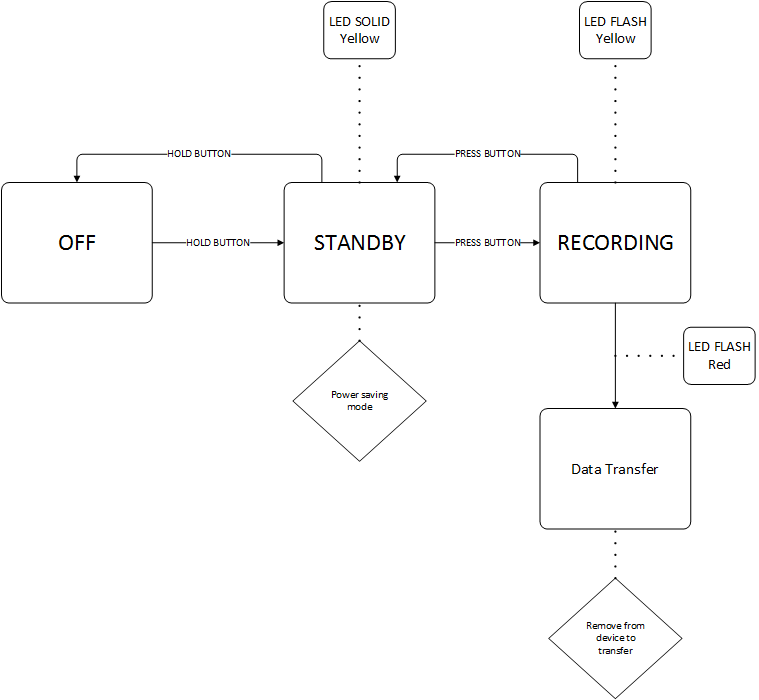
\includegraphics[width=115mm]{ImageFlow.png}
\caption{Operating Modes}
\label{overflow}
\end{figure}

\section{Exploiting the Potential}
 
 The devices have extra functionality that may or may not be used. All the devices chosen have a low power mode that will be used to out the device into 'standby'. They all have their own unique qualities, some will be discussed but overall they will not be used unless needed or will provide a great improvement to the device as it will use power.
 
\subsubsection{Micro-controller}
The micro-controller has a low power mode that will be used for the standby mode. It also supports in system debugging. This will not be used as the device will be tested and perfected and then will not receive updates or change its 'software'. It also boasts 1,000,000 read write cycles to the EEPROM. This again will not be needed at the date is wrote straight to the microSD card.

\subsubsection{Gyroscope and Accelerometer}
This particular device allows for use of either the accelerometer, the gyroscope or both. For this both will be used but the choice is optional.It also boasts a programmable interrupt device that will start the device when free fall is detected. This could be exploited in the MKII device but for the MKI device, it was built with simplicity in mind but also the ability to improve. With the sleep-to-wake and return to sleep mode, the device can be told when to go into standby mode and when to come out of standby mode. This, again, may be used in the MKII device. 

\subsubsection{Barometer}
One of the main features this provides but will not be used in a temperature sensor. It will not be used as the device is targeted for 10,000 feet and all the equipment has no problem working to -5 degrees. This may be a good feature to implement into the MKII device as it will be targeted for bigger skydives.
  
\section{Approach and Implementation to Design}
The idea was to create a prototype device device before tackling the main unit to give a better insight into how the device will be made. The prototype was made from breakout boards. This allowed focus to be given in the understanding of the how and why the components would work with each other. It also allows for a cheap and effective way to create a strong and stable working unit before sourcing out other components. The idea was to study the components from the breakout boards with the idea that they would work. they come with recommended resistors that, most probably, the company has recommended to use in sync with the devices to reduce noise. Again, this is extremely useful when building a device for the first time.
When looking at building the final device studying data sheets and the price was the key drive into the selection. Looking for key functionality and appropriate pricing would allow for the device to me made on a larger scale with a better overhead. It was also necessary to keep an eye out at extra functionary with the MKII device in mind but not essential.
  
\subsection{Debugging}
The implementation and testing of the device will be done in stages. Each sensor will run and be tested to ensure that the correct calibration and the correct data is being recorded. Making sure that the micro-controller works by running a simple, known to work, program will ensure that the other sensory equipment will recorded precisely. 
Testing each one of the components with the micro-controller and a smaller version of the final program will ensure each component works correctly. Physical testing of the equipment will also ensure that no dud readings are being stored to corrupt further data. 
All the initial testing will be done on a break out board or 'bread-board' equivalent. Then after this a PCB may be printed for the final design .

\subsubsection{Additional}
A library  may be used to call upon for the more complex areas of the code. This ties in with the amount of storage needed on the device. This is all dependent of the code needed to run and process the calculations. 
To use the device in the field it is important to understand the states the device will be in. Have the device on standby until the point of jumping, at which point put the device in to recording mode. When the device goes back into standby mode it is then ready to recoreded again, as the data has been safely moved to the microSD card. 
  
  
  
  
  
  \begin{thebibliography}{1}

  \bibitem [1] Texas Instruments, “High speed CMOS logic analog
multiplexers/demultiplexers,” 74HC4051 datasheet, Nov. 1997 [Revised Sept.
2002].

  \end{thebibliography}

 
\end{document}

